\documentclass[11pt,spanish,]{article}
\usepackage{lmodern}
\usepackage{amssymb,amsmath}
\usepackage{ifxetex,ifluatex}
\usepackage{fixltx2e} % provides \textsubscript
\ifnum 0\ifxetex 1\fi\ifluatex 1\fi=0 % if pdftex
  \usepackage[T1]{fontenc}
  \usepackage[utf8]{inputenc}
\else % if luatex or xelatex
  \ifxetex
    \usepackage{mathspec}
    \usepackage{xltxtra,xunicode}
  \else
    \usepackage{fontspec}
  \fi
  \defaultfontfeatures{Mapping=tex-text,Scale=MatchLowercase}
  \newcommand{\euro}{€}
\fi
% use upquote if available, for straight quotes in verbatim environments
\IfFileExists{upquote.sty}{\usepackage{upquote}}{}
% use microtype if available
\IfFileExists{microtype.sty}{\usepackage{microtype}}{}
\usepackage[margin=1in]{geometry}
\usepackage{color}
\usepackage{fancyvrb}
\newcommand{\VerbBar}{|}
\newcommand{\VERB}{\Verb[commandchars=\\\{\}]}
\DefineVerbatimEnvironment{Highlighting}{Verbatim}{commandchars=\\\{\}}
% Add ',fontsize=\small' for more characters per line
\newenvironment{Shaded}{}{}
\newcommand{\KeywordTok}[1]{\textcolor[rgb]{0.00,0.44,0.13}{\textbf{{#1}}}}
\newcommand{\DataTypeTok}[1]{\textcolor[rgb]{0.56,0.13,0.00}{{#1}}}
\newcommand{\DecValTok}[1]{\textcolor[rgb]{0.25,0.63,0.44}{{#1}}}
\newcommand{\BaseNTok}[1]{\textcolor[rgb]{0.25,0.63,0.44}{{#1}}}
\newcommand{\FloatTok}[1]{\textcolor[rgb]{0.25,0.63,0.44}{{#1}}}
\newcommand{\CharTok}[1]{\textcolor[rgb]{0.25,0.44,0.63}{{#1}}}
\newcommand{\StringTok}[1]{\textcolor[rgb]{0.25,0.44,0.63}{{#1}}}
\newcommand{\CommentTok}[1]{\textcolor[rgb]{0.38,0.63,0.69}{\textit{{#1}}}}
\newcommand{\OtherTok}[1]{\textcolor[rgb]{0.00,0.44,0.13}{{#1}}}
\newcommand{\AlertTok}[1]{\textcolor[rgb]{1.00,0.00,0.00}{\textbf{{#1}}}}
\newcommand{\FunctionTok}[1]{\textcolor[rgb]{0.02,0.16,0.49}{{#1}}}
\newcommand{\RegionMarkerTok}[1]{{#1}}
\newcommand{\ErrorTok}[1]{\textcolor[rgb]{1.00,0.00,0.00}{\textbf{{#1}}}}
\newcommand{\NormalTok}[1]{{#1}}
\ifxetex
  \usepackage[setpagesize=false, % page size defined by xetex
              unicode=false, % unicode breaks when used with xetex
              xetex]{hyperref}
\else
  \usepackage[unicode=true]{hyperref}
\fi
\hypersetup{breaklinks=true,
            bookmarks=true,
            pdfauthor={Miguel Anguita Ruiz; Pablo Baeyens Fernández; Pablo David Medina Sánchez; Rubén Morales Pérez; Francisco Javier Morales Piqueras},
            pdftitle={Ampliación de interpolación con Splines},
            colorlinks=true,
            citecolor=blue,
            urlcolor=blue,
            linkcolor=magenta,
            pdfborder={0 0 0}}
\urlstyle{same}  % don't use monospace font for urls
\setlength{\parindent}{0pt}
\setlength{\parskip}{6pt plus 2pt minus 1pt}
\setlength{\emergencystretch}{3em}  % prevent overfull lines
\setcounter{secnumdepth}{5}
\ifxetex
  \usepackage{polyglossia}
  \setmainlanguage{}
\else
  \usepackage[spanish]{babel}
\fi

\title{Ampliación de interpolación con Splines}
\author{Miguel Anguita Ruiz \and Pablo Baeyens Fernández \and Pablo David Medina Sánchez \and Rubén Morales Pérez \and Francisco Javier Morales Piqueras}
\usepackage{mathrsfs} \usepackage{amsthm} \usepackage{booktabs}
\usepackage{caption} \usepackage{xfrac} \usepackage{graphicx}
\newtheorem*{proposicion}{Proposición} \newtheorem*{teorema}{Teorema}
\theoremstyle{definition} \newtheorem*{definicion}{Definición}
\newtheorem*{problema}{Problema} \theoremstyle{remark}
\newtheorem*{solucion}{Solución}

\begin{document}
\maketitle

{
\hypersetup{linkcolor=black}
\setcounter{tocdepth}{3}
\tableofcontents
}
\pagebreak
\newpage
\pagebreak

\section{Splines cuadráticos}\label{splines-cuadruxe1ticos}

\subsection{Introducción a los
splines}\label{introducciuxf3n-a-los-splines}

La palabra \textbf{spline} con el tiempo se usó para referirse a una
larga banda flexible generalmente de metal, que podía usarse para
dibujar curvas continuas suaves, forzando a la banda a pasar por puntos
específicos y trazados a lo largo de dicha curva.

\begin{center}
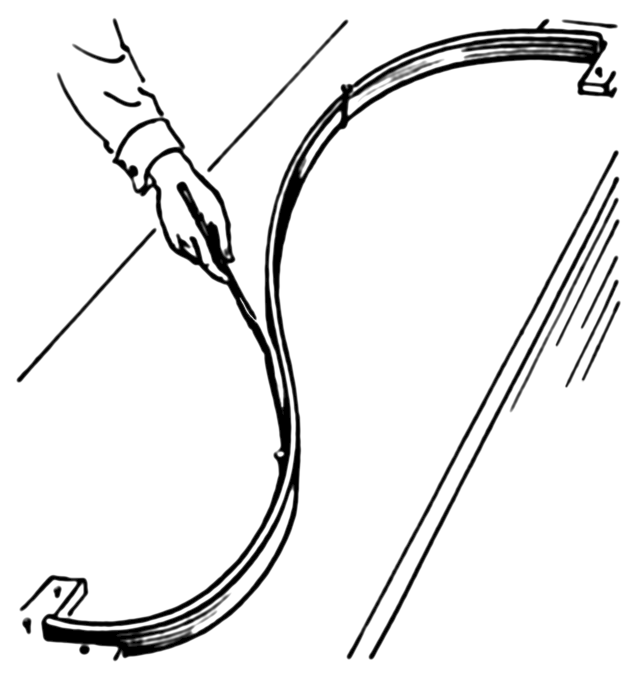
\includegraphics[scale=0.25]{spline.png}
\end{center}

La formalización del concepto de \emph{función spline}, es decir, una
curva continua que pasa por ciertos puntos se resume en la siguiente
definición:

\begin{definicion}
Sea $[a,b]$ un intervalo, $P = \{x_i\}_{i = 0...n} \in \mathscr{P}([a,b])$,
$k,r\in \mathbb{N}$, $r < k$. Se dice que $s:[a,b] \to \mathbb{R}$ es un
spline si $s \in C^r([a,b])$ y para todo $1 \leq i \leq n$,
$s_{|[x_{i-1},x_i]} \in \mathbb{P}_k$. $S^r_k(P)$ es el espacio de dichas funciones.
\end{definicion}

\vspace*{2\baselineskip}

\subsection{Descripción del espacio de splines
cuadráticos}\label{descripciuxf3n-del-espacio-de-splines-cuadruxe1ticos}

Partimos de $[a,b]$ un intervalo y $P \in \mathscr{P}([a,b])$. En esta
primera sección nos centramos en los splines cuadráticos, los
pertenecientes a $S_2^1(P)$.

Sus trozos son polinomios de grado menor o igual que $2$ de la forma
$ax^2 + bx + c$. Además son funciones de clase $1$ (derivables en
$[a,b]$ con derivada continua), lo que proporciona unas condiciones
interesantes para resolver problemas de interpolantes.

\begin{proposicion}
Sea $[a,b]$ intervalo, $P = \{x_i\}_{i=0...n} \in \mathscr{P}([a,b])$, entonces $dim(S_2(P)) = n+2$.
\end{proposicion}

\begin{proof}

Sea $s \in S_2(P)$.

- Para cada intervalo $[x_{i-1}, x_i]$ $ s|_{[x_{i-1}, x_i]}(x) = ax^2 + bx + c$ para ciertos $a,b,c \in \mathbb{R}$. Por lo tanto cada trozo está determinado por 3 parámetros. Con $n$ trozos tenemos $3n$ parámetros en total.

\pagebreak

- Si imponemos la continuidad y derivabilidad en los extremos tenemos que

\[
s_i(x_i)=s_{i+1}(x_i) \qquad s_i'(x_i)=s_{i+1}'(x_i)
\]

para todo $i=1,...,n-1$. De cada condición se obtienen $n-1$ ecuaciones, por
lo tanto obtendremos: $n-1 + n-1 = 2n-2$ ecuaciones linealmente
independientes.

Por lo tanto, $dim(S_2(P)) = 3n-(2n-2) = n+2$.
\end{proof}

Conociendo la dimensión del espacio podremos establecer una base del
espacio de splines cuadráticos con el uso de potencias truncadas. Una
\emph{base del espacio} es:

\[\{1, x, x^2, (x-x_1)_+^2, ... , (x-x_{n-1})_+^2\}\]

\vspace*{2\baselineskip}

\subsection{Interpolación con splines
cuadráticos}\label{interpolaciuxf3n-con-splines-cuadruxe1ticos}

\subsubsection{Método local: cálculo trozo a
trozo}\label{muxe9todo-local-cuxe1lculo-trozo-a-trozo}

El problema que debemos resolver es el siguiente:

\begin{problema}
Sea $[a,b]$ intervalo, $P \in \mathscr{P}([a,b])$ partición. Hallar $s \in S_2(P)$ tal que:
$$s(x_i)=y_i\ i=0,1,...,n$$
$$s'(x_k)=d_k$$
\end{problema}

Es decir, sabemos los valores de la función en todos los nodos y el
valor de la derivada en el nodo $k$.

\vspace*{2\baselineskip}

\begin{solucion}
Si $k > 0$, para calcular $s_k$ podemos calcular la tabla de diferencias divididas:
\begin{table}[h]
\centering
\begin{tabular}{llll}
x & y & DD1 & DD2\\
\hline
$x_{k-1}$ & $y_{k-1}$ & & \\
$x_k$ & $y_k$ & $p_k$ & \\
$x_k$ & $y_k$ & $d_k$ & $\frac{d_k-p_k}{h_k}$\\
\hline
\end{tabular}
\end{table}

\vspace*{2\baselineskip}
De esta forma, $s_k$ queda, para $x \in [x_{k-1}, x_k]$

\begin{equation} \label{eq:sk}
s_k(x)=y_{k-1}+p_k(x-x_{k-1})+\frac{d_k-p_k}{h_k}(x-x_{k-1})(x-x_k)
\end{equation}

Conocida la expresión de $s_k$ podemos calcular $d_{k-1} = s'_k(x_{k-1})$, y repetir
este proceso para calcular $s_{k-1}$, hasta llegar a $k = 0$.


Si $k < n$, debemos calcular $s_{k+1}$. Como sabemos la derivada $d_k$, calculamos la tabla de diferencias divididas:

\vspace*{2\baselineskip}

\begin{table}[h]
\centering
\begin{tabular}{llll}
x & y & DD1 & DD2\\
\hline
$x_k$ & $y_k$ & & \\
$x_k$ & $y_k$ & $d_k$ & \\
$x_{k+1}$ & $y_{k+1}$ & $p_{k+1}$ & $\frac{p_{k+1}-d_k}{h_k}$ \\
\hline
\end{tabular}
\end{table}

\vspace*{2\baselineskip}

De esta forma, $s_{k+1}$ queda para $x \in [x_k, x_{k+1}]$ de la siguiente forma:

\begin{equation} \label{eq:skmas}
s_{k+1}(x)=y_k+d_k(x-x_k)+\frac{p_{k+1}-d_k}{h_{k+1}}(x-x_k)(x-x_k)
\end{equation}


El método queda entonces de la siguiente forma:

\begin{enumerate}

\item Para $i$ desde $k$ hasta $0$:
\begin{enumerate}
\item Calculamos $d_i$, (conocida en el primer caso) haciendo $d_i = s'_{i+1}(x_i)$.
\item Aplicamos la fórmula (\ref{eq:sk}) para calcular $s_i$.
\end{enumerate}

\item Para $i$ desde $k+1$ hasta $n$:
\begin{enumerate}
\item Calculamos $d_i$ haciendo $d_i = s'_{i-1}(x_{i})$
\item Aplicamos la fórmula (\ref{eq:skmas}) para calcular $s_i$.
\end{enumerate}
\end{enumerate}

\end{solucion}

\vspace*{2\baselineskip}

\subsubsection{Método global: cálculo con una base de potencias
truncadas}\label{muxe9todo-global-cuxe1lculo-con-una-base-de-potencias-truncadas}

Para este método usaremos esta base del espacio vectorial $S_2(P)$:

\[\{1, x, x^2, (x-x_1)_+^2, ... , (x-x_{n-1})_+^2\}\]

Tenemos los siguientes matrices y vectores:

\begin{itemize}
\itemsep1pt\parskip0pt\parsep0pt
\item
  $G$: matriz de Gram. Evaluamos los elementos de la base en todos los
  nodos.
\item
  $X$: vector de coeficientes
\item
  $b$: vector con los valores que queremos interpolar.
\end{itemize}

De esta forma, deberíamos resolver el sistema $GX=b$.

Si notamos por $x_k$ el nodo en el que conocemos la derivada y $d_k$ la
derivada en el nodo, el sistema queda:

\begin{equation*}
\begin{pmatrix}
    1 & x_0 & x_0^2   & 0 & \cdots & 0\\
    1 & x_1 & x_1^2   & (x_1-x_1)_{+}^2 & \cdots & 0\\
    \vdots& & \vdots  & \vdots          & \cdots & \vdots \\
    \vdots& & \vdots  & \vdots          & \cdots & \vdots \\
    1 & x_n & x_n^2   & (x_n-x_1)_{+}^2 & \cdots & (x_n-x_{n-1})_{+}^2\\
    0 &   1 &  2x_k & 2(x_k-x_1)_{+} & \cdots & 2(x_k-x_{n-1})_{+}
\end{pmatrix}
\begin{pmatrix}
    a \\
    b \\
    c \\
    \alpha \\
    \vdots \\
    \omega
\end{pmatrix}
=
\begin{pmatrix}
    y_0\\
    y_1\\
    \vdots\\
    \vdots\\
    y_n\\
    d_k\\
\end{pmatrix}
\end{equation*}

Es una matriz escalonada ya que las potencias truncadas serán $0$ antes
del nodo que las define. Finalmente la solución sería, para
$x \in [a,b]$:

\[s(x) = a + bx + cx^2 + \alpha(x-x_1)_+^2 + \cdots + \omega(x-x_{n-1})_+^2\]

\subsection{Error en los splines
cuadráticos}\label{error-en-los-splines-cuadruxe1ticos}

\begin{teorema}
Sean $f \in C^2([a,b])$, $\{x_i\}_{i = 0...n} \in \mathscr{P}([a,b])$,
$s \in S_2^1(\{x_i\}_{i = 0,...,n})$ spline para $f$,

$h = max\{x_i - x_{i-1}\}_{i = 1...n}$, $E = f - s$.
Además, sea $M >0$ tal que:

\[
 M \geq Sup \{|f''(x) - f''(y)| \; : \; |x - y| \leq h, \; x,y \in [a,b] \}
 \]

Entonces, se verifica, para todo $x \in [a,b]$:

\begin{equation}
E(x) \leq \frac{h^2M}{2}
\end{equation}

\end{teorema}

La demostración, así como cotas para las derivadas y cotas más precisas
en función de la localización de $x$ puede encontrarse en
\emph{Quadratic Interpolatory Splines}, W. Kammerer, G. Reddien y R.S.
Varga, (1973).

\subsection{Ejemplos}\label{ejemplos}

\begin{problema}
Dados los datos de la tabla, halla mediante el método global el spline
cuadrático que interpole los nodos $x_i$ con $i=0,...,3$ y cuya derivada en $x_1$ sea $4$.
\begin{table}[h]
\centering
\begin{tabular}{@{}l|lllll@{}}
$x_i$ & 2 & 4 & 5 & 8 \\
$y_i$ & 7 & 3 & 5 & 5 \\
$d_i$ &   & 4 &   &   \\
\end{tabular}
\end{table}
\end{problema}

\begin{solucion}

Debemos hallar $s \in S_2(P)$ con $a,b,c, \alpha, \beta \in \mathbb{R}$ tales que, para $x \in [2,8]$:

\[ s(x)  = a + bx + cx^2 + \alpha (x - 4)^2_+ + \beta (x -5)^2_+\]

Planteamos el sistema de ecuaciones $GX = b$:

\[
\begin{pmatrix}
1 & 2 & 4  & 0  & 0\\
1 & 4 & 16 & 0  & 0\\
1 & 5 & 25 & 0  & 0\\
1 & 8 & 64 & 16 & 9\\
0 & 1 &  8 & 0  & 0
\end{pmatrix}
\begin{pmatrix}
a        \\
b        \\
c        \\
\alpha \\
\beta
\end{pmatrix}
=
\begin{pmatrix}
7\\
3\\
5\\
5\\
4
\end{pmatrix}
\]

Resolviendo el sistema, obtenemos la solución $a = 35, b = -20, c = 3, \alpha = -5, \beta = 2$. Por tanto, para $x \in [2,8]$:

\[ s(x)  = 35 - 20x + 3x^2 -5(x - 4)^2_+ + 2(x -5)^2_+\]

Es decir:

\[
s(x) =
\begin{cases}
 3x^2 - 20x + 35  & x \in [2,4] \\
-2x^2 + 20x - 45 & x \in (4,5] \\
 5  & x \in (5,8] \\
\end{cases}
\]

\end{solucion}

\begin{problema}
Dados los siguientes dados, calcula el spline cuadrático que los interpola:
\begin{table}[h]
\centering
\begin{tabular}{l|lllll}
$x_i$ & $-1$& $1$ & $3$ & $6$ & $7$ \\
$y_i$ & $1$ & $4$ & $8$ & $2$ & $9$ \\
$d_i$   &     &    & $5$ &      &     \\
\end{tabular}
\end{table}
\end{problema}

\begin{solucion}
Nos dan la derivada en el nodo 3, procedemos a calcular las diferencias divididas en los nodos 1 y 3 para hallar $s_2$:


\begin{table}[h]
\centering
\begin{tabular}{llll}
x & y & DD1 & DD2\\
\hline
$1$ & $4$ &     & \\
$3$ & $8$ & $2$ & \\
$3$ & $8$ & $5$ & $\sfrac{3}{2}$ \\
\hline
\end{tabular}
\end{table}

$s_2$ queda en su intervalo:

$$s_2(x)=4+2(x-1)+\frac{3}{2}(x-1)(x-3)$$

Ahora estimamos la derivada en el nodo 1:

$$s_2'(x)=2+\frac{3}{2}((x-3)+(x-1))=3x - 4$$

$$s_2'(1)= 3 \cdot 1 - 4 = -1$$

Realizamos de nuevo la tabla de diferencias divididas:

\begin{table}[h]
\centering
\begin{tabular}{llll}
x & y & DD1 & DD2\\
\hline
$-1$ & $1$  &                & \\
$1$  & $4$  & $\sfrac{3}{2}$  & \\
$1$  & $4$  & $-1$           & $\sfrac{-5}{4}$ \\
\hline
\end{tabular}
\end{table}

$s_1$ queda en su intervalo:

$$s_1(x)=1+\frac{3}{2}(x+1)+\frac{-5}{4}(x+1)(x-1)$$

Ahora que hemos calculado la expresión de $s$ para todos lo intervalos a la izquierda de la derivada, calculamos la función para todos los valores a la derecha de la
derivada.

Calculamos las diferencias divididas para nodos 3 y 6:

\begin{table}[h]
\centering
\begin{tabular}{llll}
x & y & DD1 & DD2\\
\hline
$3$  & $8$  &      & \\
$3$  & $8$  & $5$  & \\
$6$  & $2$  & $-2$ & $\sfrac{-7}{3}$ \\
\hline
\end{tabular}
\end{table}




$s_3$ y su derivada quedan en su intervalo:
$$s_3(x)=8+5(x-3)- \frac{7}{3} (x-3)(x-3)$$

$$s_3'(x)=5-\frac{7}{3}2(x-3)=5-\frac{7}{3}(2x-9)$$

Estimamos la derivada del nodo 6:
$$s_3'(6)=5-\frac{7}{3}3 = -2$$

Finalmente, calculamos $s_4$:

\begin{table}[h]
\centering
\begin{tabular}{llll}
x & y & DD1 & DD2\\
\hline
$6$ & $2$  &       & \\
$6$ & $2$  & $-9$  & \\
$7$ & $9$  & $7$   & $16$ \\
\hline
\end{tabular}
\end{table}

De esta forma, la expresión de $s_4$ sería:

$$s_4(x)=2 -9(x-6)+16(x-6)(x-6)$$

Por lo tanto, nuestra solución sería:


$$s(x)=
\begin{cases}
s_1(x)=1+\frac{3}{2}(x+1)+\frac{-5}{4}(x+1)(x-1)   & \text{si } x\in {[-1,1)}\\
s_2(x)=4+2(x-1)+\frac{3}{2}(x-1)(x-3)             & \text{si } x\in {[1,3)}\\
s_3(x)=8+5(x-3)- \frac{7}{3} (x-3)(x-3)           & \text{si } x\in {[3,6)}\\
s_4(x)=2 -9(x-6)+16(x-6)(x-6) & \text{si } x\in {[6,7])} \\
\end{cases}
$$
\end{solucion}

\pagebreak

\section{Splines cúbicos}\label{splines-cuxfabicos}

Uno de los problemas de la interpolación polinomial es que, al ir
aumentando el número de nodos el grado del polinomio requerido para
interpolarlos aumenta. Esto conlleva fluctuaciones en los extremos de la
interpolación.

\begin{center}
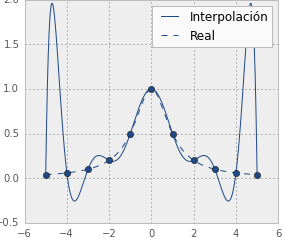
\includegraphics[scale=0.65]{problema.png}
\end{center}

Si dividimos el intervalo en una partición podemos interpolar utilizando
un polinomio S\_i(x) de grado 3 en cada intervalo, es decir, utilizando
\textbf{splines cúbicos}. Como veremos después este método minimiza la
cota de error.

\begin{equation}
    S(x) =
    \begin{cases}
    S_0(x)          & \text{si } x \in {[x_0,x_1)} \\
    S_1(x)          & \text{si } x \in {[x_1,x_2)} \\
    S_i(x)          & \text{si } x \in {[x_i,x_{i+1})} \\
    S_{n-1}(x)      & \text{si } x \in {[x_{n-1},x_n]}
    \end{cases}
\end{equation}

Esta interpolación lineal fragmentaria pasa por los puntos:
${ \{ (x_0,f(x_0)),(x_1,f(x_1)),...,(x_n,f(x_n)) \} }$

Dentro de los cúbicos encontramos los de clase 1 y 2, denotados por
$S^{1}_3$ y $S^{2}_3$ (ó $S_3$).

\begin{enumerate}
\def\labelenumi{\arabic{enumi}.}
\item
  Los splines cúbicos de \textbf{clase 1} son continuos y derivables con
  derivada continua. Conforman un espacio vectorial de dimensión
  $2(n+1)$. Una base es:
  \[\{1,x,x^2,x^3, (x-x_1)^{2}_{+},(x-x_1)^{3}_{+},...,(x-x_{n-1})^{2}_{+},(x-x_{n-1})^3_+ \}\]
  Estos splines no aseguran derivabilidad en los extremos. En un
  contexto geométrico esto significa que la función no es \emph{suave}
  en los puntos de unión. Generalmente las condiciones físicas necesitan
  esa suavidad, y es aquí donde intervienen los splines cúbicos de clase
  2.
\item
  Los splines cúbicos de \textbf{clase 2} son continuos y 2 veces
  derivables. A partir de la fórmula general, la dimensión de este
  espacio para una partición $\{x_i\}_{i=0,...,n}$ es
  $dim (S_3^2(P)) = (3-2)n+2+1=n+3$. Como tenemos $n+1$ variables,
  tenemos $2$ libertades en la resolución.
\end{enumerate}

\subsection{Construcción a partir de los valores de $S''(x)$ en los
nodos
$\{x_i\}$}\label{construcciuxf3n-a-partir-de-los-valores-de-sx-en-los-nodos-xux5fi}

Vamos a plantear un método de resolución utilizando las segundas
derivadas, denotamos, para $i=1, ..., n-1$: $M_i = S''(x_i)$, que son
desconocidos a priori salvo en un spline natural.

Como el spline es de clase 2, tenemos para $i=1, ... {n-1}$:
\[S''(x_i) = S''_i(x_i) = S''_{i+1}(x_i)\]

La restricción a cada intervalo de $S$ es un polinomio $S_i$ de grado 3,
por ende, $S''_i$ es lineal, con expresión para $x \in [x_{i-1},x_i]$:

\[S''_i(x) = M_{i-1} \frac{x_i-x}{h_i} + M_i\frac{x-x_{i-1}}{h_i}\]

Integramos dos veces usando que $S_i(x_{i-1}) = y_{i-1}$ y
$S_i(x_i) = y_i$ para las constantes de integración, obteniendo, para
${x \in [x_{i-1},x_i]}$:

\[S_i(x) = M_{i-1}\frac{(x_i-x)^3}{6h_i} + M_i\frac{x-x_{i-1}}{6h_i} + (y_{i-1}-\frac{ M_{i-1}h^2_i}{6}) \cdot \frac{x_i-x}{h_i} + (y_i-\frac{ M_ih^2_i}{6}) \cdot \frac{x-x_{i-1}}{h_i}\]

Esta ecuación nos permite calcular $S$ conocidas $M_i$ con $i=0,1,...n$.
Las condiciones de suavidad en las ligaduras nos permiten igualar
$S'_{i+1}(x_i) = S'_i(x_i)$. Derivando una vez, si
$x \in {[x_{i-1},x_i]}$:

\[S'_i(x) = -M_{i-1}\frac{(x_i-x)^2}{2h_i} + M_i\frac{(x-x_{i-1})^2}{2h_i} + \frac{y_i-y_{i-1}}{h_i} -(M_i-M_{i-1})\frac{h_i}{6}\]

Si $x \in {[x_{i},x_{i+1}]}$:

\[S'_{i+1}(x) = -M_i\frac{(x_{i+1}-x)^2}{2h_i} + M_{i+1}\frac{(x-x_i)^2}{2h_{i+1}}
 + \frac{y_{i+1}-y_i}{h_{i+1}} -(M_{i+1}-M_i)\frac{h_{i+1}}{6}\]

Recordando que $h_i = x_i - x_{i-1}$ e igualando
$S'_{i+1}(x_i) = S'_i(x_i)$:

\[-M_i\frac{h_{i+1}}{2} + \frac{y_{i+1}-y_i}{h_{i+1}} -(M_{i+1}-M_i)\frac{h_{i+1}}{6}
=  M_i\frac{h_i}{2} + \frac{y_i-y_{i-1}}{h_i} -(M_i-M_{i-1})\frac{h_i}{6}\]

Agrupamos los $M_i$:

\[-M_i\frac{h_{i+1}}{2} + M_i\frac{h_{i+1}}{6} - M_i\frac{h_i}{2} + M_i\frac{h_i}{6} + \frac{y_{i+1}-y_i}{h_{i+1}} - \frac{y_i-y_{i-1}}{h_i} =  M_{i+1}\frac{h_{i+1}}{6} + M_{i-1}\frac{h_i}{6}\]

Multiplicamos a ambos lados por $6$, sacamos factor común y recordamos
que $p_{i+1} = \frac{y_{i+1}-y_i}{h_{i+1}}$:

\[6M_i\frac{-3h_{i+1}}{6} + \frac{h_{i+1}}{6} - 3\frac{h_i}{6} + \frac{h_i}{6} + 6(p_{i+1} - p_i) =  M_{i+1}h_{i+1} + M_{i-1}h_i\]

Agrupando y multiplicando $M_i$ arriba y abajo por $-2$:

\[-2M_i\frac{-2h_{i+1}-3h_i+h_i}{-2} + 6(p_{i+1} - p_i) =  M_{i+1}h_{i+1} + M_{i-1}h_i\]

Pasamos el $M_i$ a la derecha y dividimos por $(h_{i+1}+h_i)$ en ambos
lados:

\[6\frac{p_{i+1}-p_i}{h_{i+1}+h_i} =  M_{i+1}\frac{h_{i+1}}{h_{i+1}+h_i} + M_{i-1}\frac{h_i}{h_{i+1}+h_i} + 2M_i\]

Denotando por $\displaystyle\mu_i = \frac{h_i}{h_i+h_{i+1}}$,
$\displaystyle\lambda_i = 1-\mu_i = \frac{h_{i+1}}{h_i+h_{i+1}}$ y
$\displaystyle\gamma_i = 6\frac{p_{i+1}-p_i}{h_{i+1}+h_i}$:

\begin{equation} \label{eq:ast}
\mu_iM_{i-1} + 2M_i + \lambda_iM_{i+1} = \gamma_i
\end{equation}

Con los $M_i$ en las ligaduras tendremos $4(n-1)$ variables, para que el
sistema sea determinado nos faltan dos condiciones. Hay diferentes
condiciones que se nos pueden presentar:

\vspace*{2\baselineskip}

\begin{itemize}
\itemsep1pt\parskip0pt\parsep0pt
\item
  \textbf{Spline sujeto}
\end{itemize}

$S'_1(x_0) = f'_0$ y $S'_n(x_n)=f'_n$. De acuerdo con la fórmula de
$S'(x)$ obtenemos:

\[f'_0 = -\frac{M_0h_i}{2} + f[x_0,x_1] - \frac{(M_1 - M_0)h_i}{6} \]

\[\implies  2M_0+M_1=\frac{6(f{[x_0,x_1]} - f^{'}_0)}{h_1} = 6f{[x_0,x_0,x_1]}\]

Donde el último paso se deduce de (\ref{eq:ast}). Equivalentemente para
$x_n$:

\begin{multline*}
S'_n(x_n) = - \frac{M_{n-1}(x_n-x_n)^2}{2h_n} + \frac{M_n(x_n-x_{n-1})^2}{2h_n} + \frac{(y_n-y_{n-1})}{h_n} - \frac{(M_n-M_{n-1})h_n}{6} \\
\implies
M_{n-1}+2M_n=6f[x_{n-1},x_n,x_n] (*)
\end{multline*}

Usando (*), la matriz del sistema es:

\[
\begin{pmatrix}
  2        & \lambda_0 &    0       &   \cdots  &     0          \\
  \mu_1  & 2            & \lambda_1  &   0       &    \vdots      \\
  0      & \ddots    & \ddots     &  \ddots   &     0          \\
  \vdots &     0     & \mu_{n-1}  &    2      & \lambda_{n-1}  \\
  0      &   \cdots  &     0      &   \mu_n   &     2
\end{pmatrix}
\begin{pmatrix}
  M_0 \\
  M_1 \\
  \vdots \\
  M_{n-1} \\
  M_n
\end{pmatrix} =
\begin{pmatrix}
  \gamma_0 \\
  \gamma_1 \\
  \vdots \\
  \gamma_{n-1} \\
  \gamma_n
\end{pmatrix}\]

\vspace*{2\baselineskip}

\begin{itemize}
\itemsep1pt\parskip0pt\parsep0pt
\item
  \textbf{Spline natural}
\end{itemize}

En este caso $M_0=0$ y $M_n=0$, $\lambda_0 = \mu_n = 1$ por lo que el
sistema queda:

\[\begin{pmatrix}
   2        & \lambda_1  &   0       &    \cdots     & 0 \\
  \mu_2     & 2          &  \lambda_2   &     0         & \vdots\\
  0         & \ddots     &  \ddots   &     \ddots    & 0 \\
  \vdots    &    0       & \mu_{n-2} &     2         &  \lambda_{n-2}\\
  0         &  \cdots    &    0      &    \mu_{n-1}  & 2
\end{pmatrix}
\begin{pmatrix}
  M_1 \\
  M_2 \\
  \vdots \\
  M_{n-2} \\
  M_{n-1} \\
\end{pmatrix}
=
\begin{pmatrix}
  \gamma_1 \\
  \gamma_2 \\
  \vdots \\
  \gamma_{n-2} \\
  \gamma_{n-1} \\
\end{pmatrix}\]

\vspace*{2\baselineskip}

\begin{itemize}
\itemsep1pt\parskip0pt\parsep0pt
\item
  \textbf{Spline periódico}
\end{itemize}

En este caso $S'_1(x_0) = S'_n(x_n)$ y $S''_1(x_0) = S''_n(x_n)$. El
sistema queda:

\[
\begin{pmatrix}
  2        & \lambda_0 &    0       &   \cdots  &     0          \\
  \mu_1  & 2            & \lambda_1  &   0       &    \vdots      \\
  0      & \ddots    & \ddots     &  \ddots   &     0          \\
  \vdots &     0     & \mu_{n-1}  &    2      & \lambda_{n-1}
\end{pmatrix}
\begin{pmatrix}
  M_0 \\
  M_1 \\
  \vdots \\
  M_{n-2} \\
  M_{n-1}
\end{pmatrix} =
\begin{pmatrix}
  \gamma_0=h_1-S^{'}_(x_0) \\
  \gamma_1 \\
  \vdots \\
  \gamma_{n-2} \\
  \gamma_{n-1}
\end{pmatrix}\]

En este caso añadimos:

${ S^{'}_1(x_0)= -M_0 \cdot \frac{h_1}{2}+ f{[x_o,x_1]} - \frac{M_1-M_0}{6} \cdot h_1 }$

\subsection{Propiedades de
minimización}\label{propiedades-de-minimizaciuxf3n}

Comenzamos planteando un problema de minimización sobre el espacio
euclídeo $(C^2([a,b]), <\cdot,\cdot>)$, con la métrica y norma definida
de la forma usual:

\[<f,g> = \int_a^b fg, \qquad || f || = \sqrt{ \int_a^b f^2}\]

\vspace*{\baselineskip}

Planteamos el problema:

\begin{problema}
Sea $f \in C^2([a,b])$, $P \in \mathscr{P}([a,b])$. Sea $H \subset C^2([a,b])$ definido por:
\[H = \{g \in C^2([a,b]) \; : \; \forall p \in P \; g(p) = f(p) \text{ y } \; g'(a) = f'(a), \; g'(b) = f'(b)\} \]

Hallar $u \in H$ tal que $||u''||$ sea mínima.
\end{problema}

\vspace*{\baselineskip}

Para resolver el problema, demostramos el siguiente teorema:

\begin{teorema}[Minimización]
Sea $f \in C^2([a,b])$, $P \in \mathscr{P}([a,b])$, $s$ spline sujeto para $f$. Se verifica:

\[
\forall u \in H : \; ||s''|| \leq ||u''||
\]
\end{teorema}

\vspace*{\baselineskip}

\begin{proof}
Sea $u \in H$, $e = u - s$. Tenemos:

\[
||u''||^2 = ||e'' + s''||^2 = ||e''||^2 + ||s''||^2 + 2<e'', s''>
\]

Dividimos $<e'',s''>$ en intervalos:
\[
<e'',s''> = \int_a^b e''s''
= \sum_1^{n-1} \int_{x_i}^{x_{i+1}} e''s''
\]

En cada intervalo, integramos por partes:
\[
\sum_1^{n-1}  \int_{x_i}^{x_{i+1}} e''s''
= \sum_1^{n-1}  \left. e'(x)s''(x) \right|_{x_i}^{x_{i+1}} - \sum_1^{n-1}  \int_{x_i}^{x_{i+1}}e's'''
\]

La primera sumatoria es una suma telescópica, por lo que conservamos
el primer y último término:
\[
\sum_1^{n-1} \left. e'(x)s''(x) \right|_{x_i}^{x_{i+1}}
= e'(b)s''(b) - e'(a)s''(a)
= (u'(b) - s'(b))s''(b) - (u'(a) - s'(b))s''(a)
= 0
\]

ya que $u, s \in H$.

En cuanto a la segunda, $s'''|_{[x_i, x_{i+1}]}$ es constante, por lo
que podemos sacarlo de la integral:
\[
\sum_{1}^{n-1} s_i\int_a^be' = \sum_{1}^{n-1}  s_i(e(b) - e(a)) = 0
\]

Es decir, $<e'',s''> = 0$. Por tanto:

\[
||u''||^2 = ||e''||^2 + ||s''||^2 + 2<e'', s''>
= ||e''||^2 + ||s''||^2 \geq ||s''||^2
\]

donde utilizamos que la norma siempre es positiva.
\end{proof}

Así, podemos observar que el \textbf{spline cúbico sujeto} asociado a
una función $f$ tiene la menor norma de su segunda derivada de entre las
que interpolan a $f$ en una partición dada, por lo que resuelve nuestro
problema.

\subsection{Error en los splines
cúbicos}\label{error-en-los-splines-cuxfabicos}

\begin{teorema}
Sea $f \in C^4([a,b])$, $n \in \mathbb{N}$, $P = \{x_i\}_{i = 0...n} \in \mathscr{P}([a,b])$ y  $s \in S_3^1(P)$ spline para $f$. Además, sean $h = max\{x_i - x_{i-1}\}_{i = 1...n}$, $M > 0$ cota superior de $|f^{iv)}|$ en $[a,b]$ y $E = f - s$, $x \in [a,b]$.

Se verifica:

\begin{equation} \label{eq:errorS31}
|E(x)| \leq \frac{5M}{384}h^4
\end{equation}

\end{teorema}

La demostración, así como cotas para las derivadas, puede consultarse en
\emph{Optimal Error Bounds for Cubic Spline Interpolation}, Charles Hall
y Weston Meyer, (1976).

\subsection{Ejemplos}\label{ejemplos-1}

\textbf{Sujeto}:

\begin{problema}

Hallar spline sujeto tal que:
\begin{enumerate}
\item Pasa por los puntos: $\{(0,0),(1,0.5),(2,2), (3,1.5)\}$
\item $S'(0) = 0.2$ y $S'(3) = -1$
\end{enumerate}
\end{problema}

\vspace*{\baselineskip}

\begin{solucion}
Como los nodos están equiespaciados $h_i=1$ $\forall i \in \{1..n\}$

$$\lambda_0 = \mu_3 = 1 \; \text{ y } \; \lambda_1=\lambda_2=\mu_1=\mu_2= \frac{1}{2}$$

Calculamos las diferencias divididas para obtener los $\gamma_i$

\begin{itemize}

\item $\displaystyle\frac{\gamma_0}{6} = f[x_0,x_0,x_1] =  \frac{f[x_1,x_0]-f[x_0,x_0]}{x_1-x_0} = \left(\frac{0.5-0}{1-0}-0.2\right)/1 = 0.3$

\item $\displaystyle\frac{\gamma_1}{6} = f{[x_0,x_1,x_2]} =  \frac{f{[x_2,x_1]}-f{[x_1,x_0]} }{ x_2-x_0 } = \left(\frac{2-0.5}{1-0}-\frac{0.5-0}{1-0}\right)/2 = \frac{1}{2}$

\item $\displaystyle\frac{\gamma_2}{6} = f{[x_1,x_2,x_3]} =  \frac{ f{[x_3,x_2]}-f{[x_2,x_1]} }{ x_3-x_1 } = \left(\frac{1.5-2}{1-0}-\frac{2-0.5}{1-0}\right)/1 = -1$

\item $\displaystyle\frac{\gamma_3}{6} = f{[x_2,x_3,x_3]} =  \frac{ f{[x_3,x_3]}-f{[x_2,x_3]} }{ x_3-x_2 } = \left(-1-\frac{1.5-2}{1-0}\right)/1 = -\frac{1}{2}$
\end{itemize}

El sistem queda:

\begin{equation*}
\begin{pmatrix}
    2 & 1 & 0 & 0  \\
    1/2 & 2 & 1/2 & 0  \\
    0 & 1/2 & 2 & 1/2  \\
    0 & 0 & 1 & 1/2
\end{pmatrix}
\begin{pmatrix}
    M_0  \\
    M_1  \\
    M_2  \\
    M_3
\end{pmatrix}
=
\begin{pmatrix}
    6\cdot\frac{3}{10}  \\
    6\cdot\frac{1}{2}  \\
    6\cdot(-1)  \\
    6\cdot(-\frac{1}{2})
\end{pmatrix}
\end{equation*}

Del que obtenemos la solución $M_0=-0.36, M_1=2.52, M_2=-3.72 \text{ y } M_3=0.36$.
Calculamos los trozos finalmente aplicando la fórmula:

$$S_1(x)= M_0\frac{(x_1-x)^3}{6} + M_1\frac{(x-x_0)^3}{6} + (y_0-\frac{M_0}{6})\frac{x_1-x}{1} + (y_1-\frac{M_1}{6})\frac{x-x_0}{1} = 0.48x^3 - 0.18x^2 + 0.2x$$

Equivalentemente para $S_2$ y $S_3$, obtenemos la solución:

\begin{equation*}
 S(x) =
  \begin{cases}
   0.48x^3 - 0.18x^2 + 0.2x &                              \text{si } 0 \leq x \leq 1  \\
   -1.04x(x-1)^3 + 1.26(x-1)^2 + 1.28(x-1) - 0.5   &  \text{si } 1 < x \leq 2  \\
   0.68(x-2)^3 - 1.86(x-2)^2 + 0.68(x-2) + 2       &  \text{si } 2 < x \leq 3  \\
  \end{cases}
\end{equation*}
\end{solucion}

\textbf{Natural}:

\begin{problema}
Hallar spline natural tal que:
\begin{enumerate}
\item Pasa por los puntos: $\{(1,3),(2,6),(3,4), (4,0)\}$
\item $S^{'}(0) = S^{'}(3)$ y $S{''}(0) = S^{''}(3)$
\end{enumerate}
\end{problema}

\vspace*{\baselineskip}

\begin{solucion}
Como los nodos están equiespaciados $h_i=1$ $\forall i \in \{1..n\}$

$$ \mu_2 = \lambda_1 =\frac{1}{2} $$

Calculamos las diferencias divididas para obtener los $\gamma_i$

\begin{itemize}

\item $\displaystyle\frac{\gamma_1}{6}=f{[x_0,x_1,x_2]}=\frac{f{[x_2,x_1]}-f{[x_1,x_0]} }{ x_2-x_0 }=\left(\frac{4-6}{3-2}-\frac{6-3}{2-1}\right)/2=-\frac{5}{2}$

\item $\displaystyle\frac{\gamma_2}{6}=f{[x_1,x_2,x_3]}=\frac{ f{[x_3,x_2]}-f{[x_2,x_1]} }{ x_3-x_1 }=\left(\frac{0-4}{4-3}-\frac{4-6}{3-2}\right)/2=-1$

\end{itemize}

El sistem queda:

\begin{equation*}
\begin{pmatrix}
    2 & 1/2 \\
    1/2 & 2 
\end{pmatrix}
\begin{pmatrix}
    M_1  \\
    M_2  
\end{pmatrix}
=
\begin{pmatrix}
    6\cdot(-\frac{5}{2})  \\
    6\cdot(-1) 
\end{pmatrix}
\end{equation*}

Del que obtenemos la solución $M_1=-\frac{36}{5}$, $M_2= -\frac{6}{5}$.
Calculamos los trozos finalmente aplicando la fórmula:

$$S_1(x)= M_0\frac{(x_1-x)^3}{6} + M_1\frac{(x-x_0)^3}{6} + (y_0-\frac{M_0}{6})\cdot\frac{x_1-x}{1} + (y_1-\frac{M_1}{6})\cdot\frac{x-x_0}{1} = 0.48x^3 - 0.18x^2 + 0.2x$$

Equivalentemente para $S_2$ y $S_3$, obtenemos la solución:

\begin{equation*}
 S(x) =
  \begin{cases}
   1.2x^3 + 3.6x^2 + \frac{3}{5}x &                                \text{si } 1 \leq x \leq 2  \\
   x^3-\frac{48}{5}x^2+\frac{159}{5}x -32   &  \text{si } 2 < x \leq 3  \\
   \frac{6}{5}x^3-\frac{72}{5}x^2+\frac{267}{5}x-60  &  \text{si } 3 < x \leq 4  \\
  \end{cases}
\end{equation*}
\end{solucion}

\pagebreak

\section{Implementación en ordenador:
Octave}\label{implementaciuxf3n-en-ordenador-octave}

\subsection{Spline lineal}\label{spline-lineal}

La implementación de la función que nos permite calcular un spline
lineal es muy sencilla:

\begin{Shaded}
\begin{Highlighting}[]
\NormalTok{function s = SplineLineal(x,y)}
  \NormalTok{p = }\FunctionTok{diff}\NormalTok{(y)./}\FunctionTok{diff}\NormalTok{(x);}
  \NormalTok{A = [p' y(}\FloatTok{1}\NormalTok{:end-}\FloatTok{1}\NormalTok{)'];}
  \NormalTok{s = }\FunctionTok{mkpp}\NormalTok{(x,A);}
\NormalTok{end}
\end{Highlighting}
\end{Shaded}

\subsection{Splines cuadráticos}\label{splines-cuadruxe1ticos-1}

Utilizando el \textbf{método global}, podemos definir fácilmente una
función que calcule un spline cuadrático de clase 1:

\begin{Shaded}
\begin{Highlighting}[]
\NormalTok{function s = SplineCuad(x, y, d_k, k)}
  \NormalTok{# Número de intervalos}
  \NormalTok{n = }\FunctionTok{length}\NormalTok{(x) - }\FloatTok{1}\NormalTok{;}

  \CommentTok{# 1, x, x^2}
  \NormalTok{A(:,}\FloatTok{1}\NormalTok{) = [}\FunctionTok{ones}\NormalTok{(n+}\FloatTok{1}\NormalTok{,}\FloatTok{1}\NormalTok{); }\FloatTok{0}\NormalTok{];}
  \NormalTok{A(:,}\FloatTok{2}\NormalTok{) = [x'         ; }\FloatTok{1}\NormalTok{];}
  \NormalTok{A(:,}\FloatTok{3}\NormalTok{) = [x'.^}\FloatTok{2}      \NormalTok{; }\FloatTok{2}\NormalTok{.*x(k+}\FloatTok{1}\NormalTok{)];}

  \CommentTok{# Potencias truncadas}
  \NormalTok{for }\BaseNTok{j} \NormalTok{= }\FloatTok{4} \NormalTok{: n + }\FloatTok{2}
    \NormalTok{t       =  @(s) (s > x(}\BaseNTok{j}\NormalTok{-}\FloatTok{2}\NormalTok{)) .* (s - x(}\BaseNTok{j}\NormalTok{-}\FloatTok{2}\NormalTok{));}
    \NormalTok{A(:, }\BaseNTok{j}\NormalTok{) = [t(x').^}\FloatTok{2}\NormalTok{; }\FloatTok{2}\NormalTok{.*t(x(k+}\FloatTok{1}\NormalTok{))];}
  \NormalTok{end}

  \NormalTok{# Resolución del sistema}
  \NormalTok{sol = A \textbackslash{} [y' ; d_k];}

  \NormalTok{for k = }\FloatTok{1}\NormalTok{:n}
    \NormalTok{p = sol(}\FloatTok{3}\NormalTok{:-}\FloatTok{1}\NormalTok{:}\FloatTok{1}\NormalTok{);}

    \NormalTok{for l = }\FloatTok{2}\NormalTok{:k}
      \NormalTok{p += sol(l+}\FloatTok{2}\NormalTok{).*[}\FloatTok{1}\NormalTok{, -}\FloatTok{2}\NormalTok{.*x(l), x(l).^}\FloatTok{2}\NormalTok{];}
    \NormalTok{end}

    \NormalTok{B(k, :) = polyaffine(p,[-x(k) }\FloatTok{1}\NormalTok{]);}
  \NormalTok{end}

  \NormalTok{s = }\FunctionTok{mkpp}\NormalTok{(x,B);}
\NormalTok{end}
\end{Highlighting}
\end{Shaded}

Otra implementación posible es calcular el spline \textbf{a trozos}:

\begin{Shaded}
\begin{Highlighting}[]
\NormalTok{function z = SplineCuadLocal(x, y, d_k, k)}
    \NormalTok{s = }\FunctionTok{zeros}\NormalTok{(}\FunctionTok{length}\NormalTok{(x)-}\FloatTok{1}\NormalTok{, }\FloatTok{3}\NormalTok{);}
  \NormalTok{d = d_k;}
  \CommentTok{#Recorremos todos los nodos de n+1 en adelante:}

  \NormalTok{for }\BaseNTok{i} \NormalTok{= (k+}\FloatTok{1}\NormalTok{):(}\FunctionTok{length}\NormalTok{(x)-}\FloatTok{1}\NormalTok{)}
        \NormalTok{p = (y(}\BaseNTok{i}\NormalTok{+}\FloatTok{1}\NormalTok{)-y(}\BaseNTok{i}\NormalTok{))/(x(}\BaseNTok{i}\NormalTok{+}\FloatTok{1}\NormalTok{)-x(}\BaseNTok{i}\NormalTok{));}
        \NormalTok{q = (p-d)/(x(}\BaseNTok{i}\NormalTok{+}\FloatTok{1}\NormalTok{)-x(}\BaseNTok{i}\NormalTok{));}
        \NormalTok{v = [x(}\BaseNTok{i}\NormalTok{) x(}\BaseNTok{i}\NormalTok{)];}
        \NormalTok{s(}\BaseNTok{i}\NormalTok{,:) = [}\FloatTok{0}\NormalTok{, }\FloatTok{0}\NormalTok{, y(}\BaseNTok{i}\NormalTok{)]+[}\FloatTok{0}\NormalTok{, d, -d*x(}\BaseNTok{i}\NormalTok{)]+q*}\FunctionTok{poly}\NormalTok{(v);}
        \NormalTok{d = }\FunctionTok{polyval}\NormalTok{(}\FunctionTok{polyder}\NormalTok{(s(}\BaseNTok{i}\NormalTok{,:)),x(}\BaseNTok{i}\NormalTok{+}\FloatTok{1}\NormalTok{));}
    \NormalTok{end}
    \NormalTok{d = d_k;}

  \CommentTok{#Recorremos todos los nodos desde n hasta el 1:}

  \NormalTok{for }\BaseNTok{j} \NormalTok{= k:-}\FloatTok{1}\NormalTok{:}\FloatTok{1}
        \NormalTok{p = (y(}\BaseNTok{j}\NormalTok{+}\FloatTok{1}\NormalTok{)-y(}\BaseNTok{j}\NormalTok{))/(x(}\BaseNTok{j}\NormalTok{+}\FloatTok{1}\NormalTok{)-x(}\BaseNTok{j}\NormalTok{))}
        \NormalTok{q = (d-p)/(x(}\BaseNTok{j}\NormalTok{+}\FloatTok{1}\NormalTok{)-x(}\BaseNTok{j}\NormalTok{))}
        \NormalTok{v = [x(}\BaseNTok{j}\NormalTok{) x(}\BaseNTok{j}\NormalTok{+}\FloatTok{1}\NormalTok{)]}
        \NormalTok{s(}\BaseNTok{j}\NormalTok{,:) = [}\FloatTok{0} \FloatTok{0} \NormalTok{y(}\BaseNTok{j}\NormalTok{)]+[}\FloatTok{0} \NormalTok{p -p*x(}\BaseNTok{j}\NormalTok{)]+q*}\FunctionTok{poly}\NormalTok{(v);}
        \NormalTok{d = }\FunctionTok{polyval}\NormalTok{(}\FunctionTok{polyder}\NormalTok{(s(}\BaseNTok{j}\NormalTok{,:)), x(}\BaseNTok{j}\NormalTok{))}
  \NormalTok{end}

  \NormalTok{for }\BaseNTok{i} \NormalTok{= }\FloatTok{1}\NormalTok{:}\FunctionTok{length}\NormalTok{(s)}
    \NormalTok{s(}\BaseNTok{i}\NormalTok{,:) = polyaffine(s(}\BaseNTok{i}\NormalTok{,:), [-x(}\BaseNTok{i}\NormalTok{), }\FloatTok{1}\NormalTok{]);}
  \NormalTok{end}
    \NormalTok{z = }\FunctionTok{mkpp}\NormalTok{(x, s);}
\NormalTok{end}
\end{Highlighting}
\end{Shaded}

\subsection{Splines cúbicos}\label{splines-cuxfabicos-1}

Para el cálculo de splines cúbicos por medio de la segunda derivada nos
hemos valido de la interpolación de splines lineales y de la función
\texttt{ppint}, que realiza la integración de un spline.

\subsubsection{Spline sujeto}\label{spline-sujeto}

La función para el cálculo del \textbf{spline sujeto} queda:

\begin{Shaded}
\begin{Highlighting}[]
\NormalTok{function s = SplineSuj (x, y, d_1, d_n)}
  \NormalTok{n     = }\FunctionTok{length}\NormalTok{(x) - }\FloatTok{1}\NormalTok{;}
  \NormalTok{twoes = }\FloatTok{2}\NormalTok{*}\FunctionTok{ones}\NormalTok{(}\FloatTok{1}\NormalTok{,n+}\FloatTok{1}\NormalTok{);}
  \NormalTok{h     = }\FunctionTok{diff}\NormalTok{(x);}

  \NormalTok{mu     = [(h(}\FloatTok{1}\NormalTok{:end-}\FloatTok{1}\NormalTok{)./(h(}\FloatTok{1}\NormalTok{:end-}\FloatTok{1}\NormalTok{) + h(}\FloatTok{2}\NormalTok{:end))) }\FloatTok{1}\NormalTok{];}
  \NormalTok{lambda = }\FunctionTok{ones}\NormalTok{(}\FloatTok{1}\NormalTok{,n) - [}\FloatTok{0} \NormalTok{mu(}\FloatTok{1}\NormalTok{:end-}\FloatTok{1}\NormalTok{)];}

  \NormalTok{A = }\FunctionTok{diag}\NormalTok{(mu,-}\FloatTok{1}\NormalTok{) + }\FunctionTok{diag}\NormalTok{(twoes,}\FloatTok{0}\NormalTok{) + }\FunctionTok{diag}\NormalTok{(lambda,}\FloatTok{1}\NormalTok{);}

  \NormalTok{dd1 = }\FunctionTok{diff}\NormalTok{(y)./h;}
  \NormalTok{for }\BaseNTok{i}\NormalTok{=}\FloatTok{1}\NormalTok{:(n-}\FloatTok{1}\NormalTok{)}
          \NormalTok{dd2(}\BaseNTok{i}\NormalTok{)=(dd1(}\BaseNTok{i}\NormalTok{+}\FloatTok{1}\NormalTok{)-dd1(}\BaseNTok{i}\NormalTok{))/(x(}\BaseNTok{i}\NormalTok{+}\FloatTok{2}\NormalTok{)-x(}\BaseNTok{i}\NormalTok{));}
  \NormalTok{end}

  \FunctionTok{gamma}\NormalTok{(}\FloatTok{1}\NormalTok{)   = }\FloatTok{6}\NormalTok{*(dd2(}\FloatTok{1}\NormalTok{)-d_1)/(x(}\FloatTok{2}\NormalTok{)-x(}\FloatTok{1}\NormalTok{));}
  \FunctionTok{gamma}\NormalTok{(}\FloatTok{2}\NormalTok{:n) = }\FloatTok{6}\NormalTok{*dd2(}\FloatTok{1}\NormalTok{:n-}\FloatTok{1}\NormalTok{);}
  \FunctionTok{gamma}\NormalTok{(n+}\FloatTok{1}\NormalTok{) = }\FloatTok{6}\NormalTok{*(d_n-dd2(n-}\FloatTok{1}\NormalTok{))/(x(n+}\FloatTok{1}\NormalTok{)-x(n));}

  \NormalTok{m = A\textbackslash{}gamma';}
  \NormalTok{s = ppint(ppint(SplineLineal(x, m')));}
\NormalTok{end}
\end{Highlighting}
\end{Shaded}

\subsubsection{Spline natural}\label{spline-natural}

Para el \textbf{spline natural} calculamos la matriz, resolvemos el
sistema e integramos añadiendo los datos de las derivadas segundas en
los extremos:

\begin{Shaded}
\begin{Highlighting}[]
\NormalTok{function s = SplineNat(x, y)}
  \NormalTok{n = }\FunctionTok{length}\NormalTok{(x) - }\FloatTok{1}\NormalTok{;}

  \NormalTok{h = }\FunctionTok{diff}\NormalTok{(x);     }\CommentTok{#h_i}
  \NormalTok{p = }\FunctionTok{diff}\NormalTok{(y)./h;  }\CommentTok{#p_i}

  \NormalTok{twoes  = }\FloatTok{2}\NormalTok{*}\FunctionTok{ones}\NormalTok{(}\FloatTok{1}\NormalTok{,n-}\FloatTok{1}\NormalTok{);}
  \NormalTok{mu     = (h(}\FloatTok{1}\NormalTok{:end-}\FloatTok{1}\NormalTok{)./(h(}\FloatTok{1}\NormalTok{:end-}\FloatTok{1}\NormalTok{) + h(}\FloatTok{2}\NormalTok{:end)));}
  \NormalTok{lambda = }\FunctionTok{ones}\NormalTok{(}\FloatTok{1}\NormalTok{,n-}\FloatTok{1}\NormalTok{) - mu;}
  \FunctionTok{gamma}  \NormalTok{= }\FunctionTok{diff}\NormalTok{(p)./(h(}\FloatTok{1}\NormalTok{:end-}\FloatTok{1}\NormalTok{) + h(}\FloatTok{2}\NormalTok{:end));}

  \NormalTok{if(n < }\FloatTok{3}\NormalTok{)}
    \NormalTok{A = }\FloatTok{2}\NormalTok{;}
  \NormalTok{else}
    \NormalTok{A = }\FunctionTok{diag}\NormalTok{(twoes) + }\FunctionTok{diag}\NormalTok{(lambda(}\FloatTok{1}\NormalTok{:end-}\FloatTok{1}\NormalTok{),}\FloatTok{1}\NormalTok{) + }\FunctionTok{diag}\NormalTok{(mu(}\FloatTok{2}\NormalTok{:end),-}\FloatTok{1}\NormalTok{);}
  \NormalTok{end}

  \NormalTok{m = A \textbackslash{} gamma';}
  \NormalTok{s = ppint(ppint(SplineLineal(x, [}\FloatTok{0} \NormalTok{m' }\FloatTok{0}\NormalTok{])));}
\NormalTok{end}
\end{Highlighting}
\end{Shaded}

\subsubsection{Spline periódico}\label{spline-periuxf3dico}

La función del \textbf{spline periódico} queda:

\begin{Shaded}
\begin{Highlighting}[]
\NormalTok{function z = SplinePer (x, y)}
        \NormalTok{n=}\FunctionTok{length}\NormalTok{(x);}
        \NormalTok{twoes=}\FloatTok{2}\NormalTok{*}\FunctionTok{ones}\NormalTok{(}\FloatTok{1}\NormalTok{,n);}
        \NormalTok{h=}\FunctionTok{diff}\NormalTok{(x);}
        \NormalTok{lambda=[}\FloatTok{1}\NormalTok{];}
        \NormalTok{for }\BaseNTok{i}\NormalTok{=}\FloatTok{1}\NormalTok{:(n-}\FloatTok{2}\NormalTok{)}
                \NormalTok{lambda(}\BaseNTok{i}\NormalTok{+}\FloatTok{1}\NormalTok{)=h(}\BaseNTok{i}\NormalTok{+}\FloatTok{1}\NormalTok{)/(h(}\BaseNTok{i}\NormalTok{+}\FloatTok{1}\NormalTok{)+h(}\BaseNTok{i}\NormalTok{));}
        \NormalTok{endfor}
        \NormalTok{mu=[];}
        \NormalTok{for }\BaseNTok{i}\NormalTok{=}\FloatTok{1}\NormalTok{:(n-}\FloatTok{2}\NormalTok{)}
                \NormalTok{mu(}\BaseNTok{i}\NormalTok{)=h(}\BaseNTok{i}\NormalTok{)/(h(}\BaseNTok{i}\NormalTok{+}\FloatTok{1}\NormalTok{)+h(}\BaseNTok{i}\NormalTok{));}
        \NormalTok{endfor}
        \NormalTok{mu(n-}\FloatTok{1}\NormalTok{)=}\FloatTok{1}\NormalTok{;}
        \NormalTok{A=}\FunctionTok{diag}\NormalTok{(mu,-}\FloatTok{1}\NormalTok{)+}\FunctionTok{diag}\NormalTok{(twoes,}\FloatTok{0}\NormalTok{)+}\FunctionTok{diag}\NormalTok{(lambda,}\FloatTok{1}\NormalTok{);}
        \NormalTok{dd1=}\FunctionTok{zeros}\NormalTok{(n-}\FloatTok{1}\NormalTok{,}\FloatTok{1}\NormalTok{);}
        \NormalTok{for }\BaseNTok{i}\NormalTok{=}\FloatTok{1}\NormalTok{:(n-}\FloatTok{1}\NormalTok{)}
                \NormalTok{dd1(}\BaseNTok{i}\NormalTok{)=(y(}\BaseNTok{i}\NormalTok{+}\FloatTok{1}\NormalTok{)-y(}\BaseNTok{i}\NormalTok{))/(x(}\BaseNTok{i}\NormalTok{+}\FloatTok{1}\NormalTok{)-x(}\BaseNTok{i}\NormalTok{));}
        \NormalTok{endfor}
        \NormalTok{dd2=}\FunctionTok{zeros}\NormalTok{(n-}\FloatTok{2}\NormalTok{,}\FloatTok{1}\NormalTok{);}
        \NormalTok{for }\BaseNTok{i}\NormalTok{=}\FloatTok{1}\NormalTok{:(n-}\FloatTok{2}\NormalTok{)}
                \NormalTok{dd2(}\BaseNTok{i}\NormalTok{)=(dd1(}\BaseNTok{i}\NormalTok{+}\FloatTok{1}\NormalTok{)-dd1(}\BaseNTok{i}\NormalTok{))/(x(}\BaseNTok{i}\NormalTok{+}\FloatTok{2}\NormalTok{)-x(}\BaseNTok{i}\NormalTok{));}
        \NormalTok{endfor}
   \NormalTok{A(}\FloatTok{1}\NormalTok{,:)=h(}\FloatTok{1}\NormalTok{)*A(}\FloatTok{1}\NormalTok{,:);}
   \NormalTok{A(}\FloatTok{1}\NormalTok{,}\FloatTok{1}\NormalTok{)=A(}\FloatTok{1}\NormalTok{,}\FloatTok{1}\NormalTok{)-h(}\FloatTok{1}\NormalTok{)/}\FloatTok{3}\NormalTok{;}
   \NormalTok{A(}\FloatTok{1}\NormalTok{,}\FloatTok{2}\NormalTok{)=A(}\FloatTok{1}\NormalTok{,}\FloatTok{2}\NormalTok{)+h(}\FloatTok{1}\NormalTok{)/}\FloatTok{6}\NormalTok{;}
   \NormalTok{A(n,:)=h(n-}\FloatTok{1}\NormalTok{)*A(}\FloatTok{1}\NormalTok{,:);}

   \NormalTok{A(n,}\FloatTok{1}\NormalTok{)=A(}\FloatTok{1}\NormalTok{,}\FloatTok{1}\NormalTok{)+h(}\FloatTok{1}\NormalTok{)/}\FloatTok{3}\NormalTok{;}
   \NormalTok{A(n,}\FloatTok{2}\NormalTok{)=A(}\FloatTok{1}\NormalTok{,}\FloatTok{2}\NormalTok{)-h(}\FloatTok{1}\NormalTok{)/}\FloatTok{6}\NormalTok{;}
   \FunctionTok{gamma}\NormalTok{=}\FunctionTok{zeros}\NormalTok{(n,}\FloatTok{1}\NormalTok{);}
        \FunctionTok{gamma}\NormalTok{(}\FloatTok{1}\NormalTok{)=h(}\FloatTok{1}\NormalTok{)-dd1(}\FloatTok{1}\NormalTok{);}
   \FunctionTok{gamma}\NormalTok{(n)=-h(n-}\FloatTok{1}\NormalTok{)+dd1(}\FloatTok{1}\NormalTok{);}
        \NormalTok{for }\BaseNTok{i}\NormalTok{=}\FloatTok{1}\NormalTok{:(n-}\FloatTok{2}\NormalTok{)}
                \FunctionTok{gamma}\NormalTok{(}\BaseNTok{i}\NormalTok{+}\FloatTok{1}\NormalTok{)=}\FloatTok{6}\NormalTok{*dd2(}\BaseNTok{i}\NormalTok{);}
        \NormalTok{endfor}
   \NormalTok{m=A\textbackslash{}}\FunctionTok{gamma}\NormalTok{;}
    \NormalTok{s = ppint(ppint(SplineLineal(x, m)));}
\NormalTok{end}
\end{Highlighting}
\end{Shaded}

\pagebreak
\appendix

\section{Definiciones y notación}\label{definiciones-y-notaciuxf3n}

\begin{definicion}
Sea $I \subset \mathbb{R}$ un intervalo cerrado y acotado con extremos $a,b$:

\begin{itemize}
\item Una \textbf{partición} $P$ de $I$ es un subconjunto finito de $I$ con $a,b\in P$ .
\item $\mathscr{P}(I)$ es el conjunto de todas las particiones de $I$.
\end{itemize}
\end{definicion}

\vspace*{3pt}

\begin{definicion} Sea $a \in \mathbb{R}$, $n \in \mathbb{N}$. La
\textbf{potencia truncada} en $a$ de grado $n$, $(x - a)_+^n$ viene dada por:

\[
 (x - a)_+^n =
  \begin{cases}
      0             & \text{si } x \leq a \\
   (x - a)^n   & \text{si } x > a
  \end{cases}
\]
\end{definicion}

Cualquier potencia truncada de grado $n$ es de clase $n - 1$, y su
derivada de orden $n$ presenta una discontinuidad en $a$. La derivada de
$(x - a)_+^n$ en $x$ es $n(x - a)_+^{n-1}$.

Su implementación en Octave es bastante sencilla: dados \texttt{a} y
\texttt{n}, podemos definir la potencia truncada como función anónima de
la siguiente forma:

\begin{Shaded}
\begin{Highlighting}[]
\NormalTok{pot = @(x) (x > a) * (x - a)^n}
\end{Highlighting}
\end{Shaded}

Como Octave tiene tipos dinámicos convertirá
\texttt{(x \textgreater{} a)} a $1$ si $x > a$ y a $0$ en otro caso.

\begin{definicion}
Dado un intervalo $[a,b]$ y una partición $\{x_i\}_{i = 0...n} \in \mathscr{P}([a,b])$,
se definen, para $1 \leq i \leq n$:

\begin{itemize}
\item $\displaystyle h_i = x_i - x_{i-1}$
\item $\displaystyle p_i = \frac{y_i-y_{i-1}}{h_i}$
\end{itemize}
\end{definicion}

\section{Bibliografía}\label{bibliografuxeda}

\begin{itemize}
\itemsep1pt\parskip0pt\parsep0pt
\item
  \href{http://www.math.kent.edu/~varga/pub/paper_85.pdf}{\emph{Quadratic
  Interpolatory Splines} - W.J.Kammerer, G. W. Reddien, and R.S. Varga}
\item
  \href{https://en.wikiversity.org/wiki/Cubic_Spline_Interpolation}{\emph{Cubic
  Spline Interpolation}}
  (https://en.wikiversity.org/wiki/Cubic\_Spline\_Interpolation)
\item
  \emph{Análisis numérico (Novena Edición)} - Richard L. Burden y J.
  Douglas Faires
\item
  \emph{Analysis of Numerical Methods} - Eugene Isaacson, Herbert Bishop
  Keller
\item
  \emph{Spline Approximation of Functions and Data} - Universidad de
  Oslo
\item
  \emph{Optimal Error Bounds for Cubic Spline Interpolation} - Charles
  A. Hall
\end{itemize}

\end{document}
